\chapter{Gradients of all architectures - shifted}\label{appendixB}

\section*{Velocity}\label{sec:velocity-appendixB}

\subsection*{Full dataset}\label{subsec:vel-full-dataset-appendixB}
\begin{figure}[!htpb]
\centering
\begin{subfigure}[b]{\textwidth}
   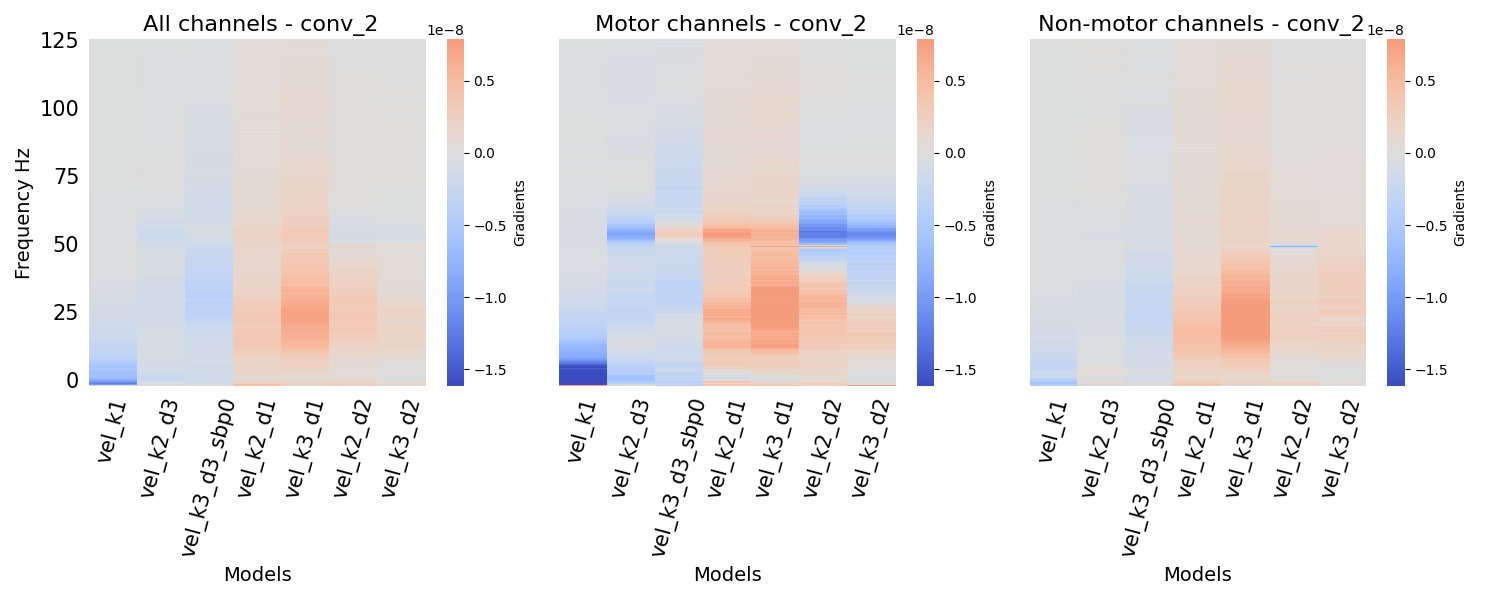
\includegraphics[width=0.85\linewidth]{img/appendix/A/conv-2/sm/vel-model-gradients-all_kinds}
   \caption{}
   \label{fig:vel-shifted-grads-conv-2}
\end{subfigure}

\begin{subfigure}[b]{\textwidth}
   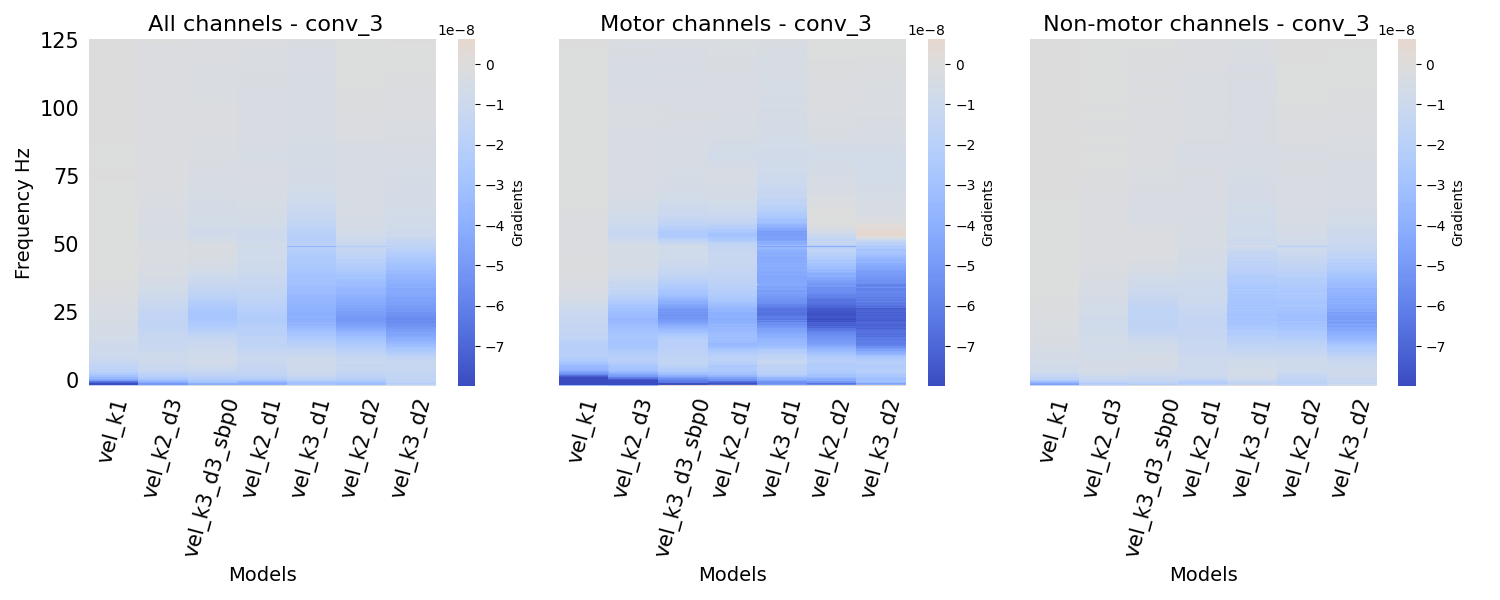
\includegraphics[width=0.85\linewidth]{img/appendix/A/conv-3/sm/vel-model-gradients-all_kinds}
   \caption{}
   \label{fig:vel-shifted-grads-conv-3}
\end{subfigure}
\end{figure}
\clearpage   

\begin{figure}[!htbp]\ContinuedFloat

\begin{subfigure}[b]{\textwidth}
   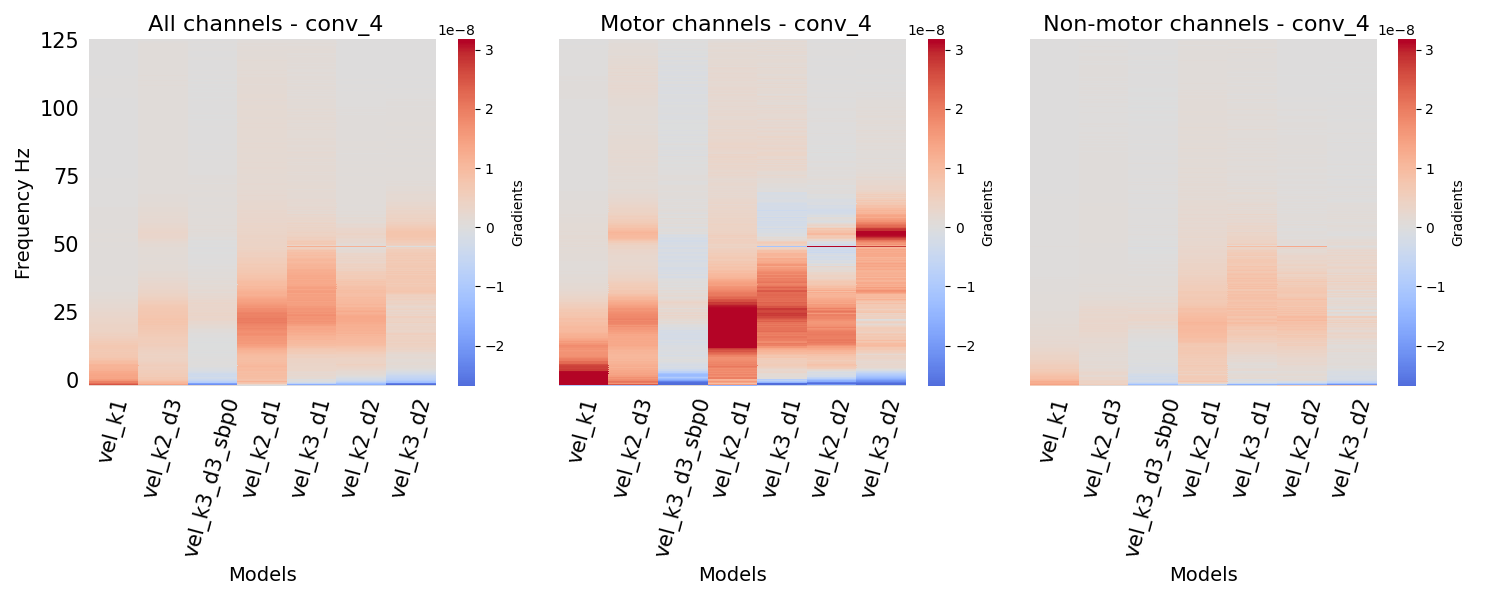
\includegraphics[width=1\linewidth]{img/appendix/A/conv-4/sm/vel-model-gradients_all_kinds}
   \caption{}
   \label{fig:vel-shifted-grads-conv-4}
\end{subfigure}

\begin{subfigure}[b]{\textwidth}
   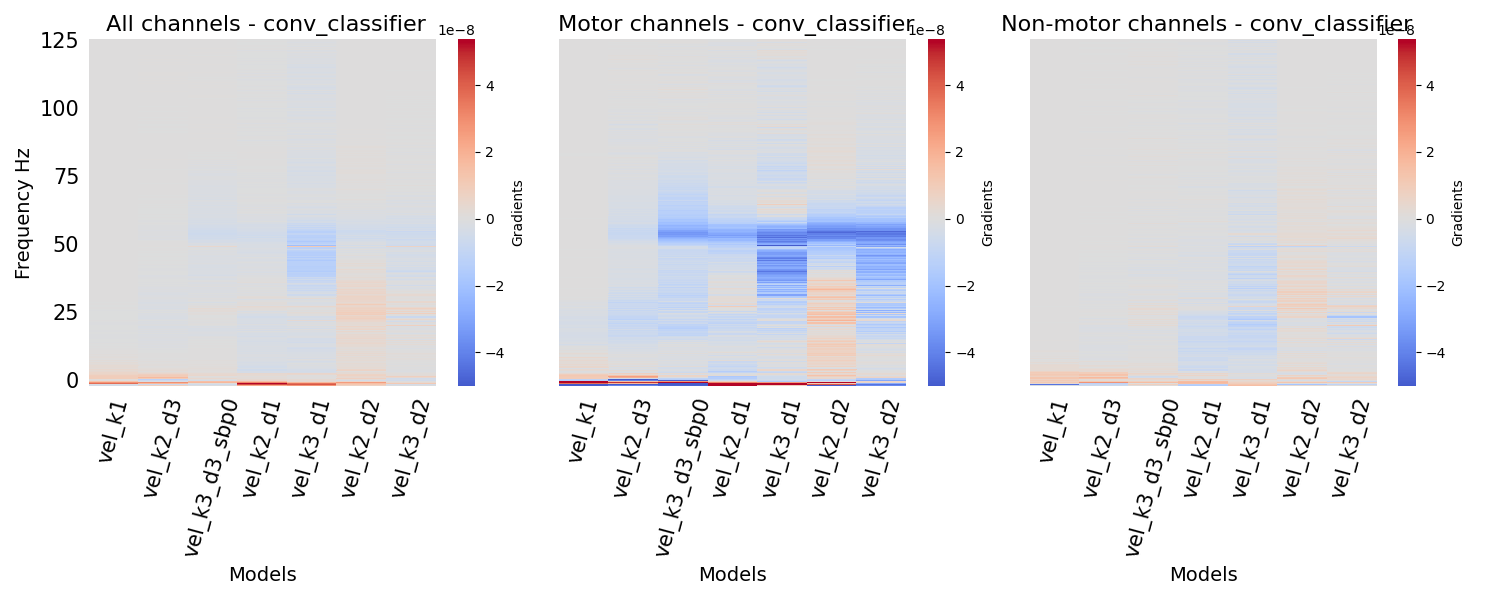
\includegraphics[width=1\linewidth]{img/appendix/A/conv-classifier/sm/vel-model-gradients_all_kinds}
   \caption{}
   \label{fig:vel-shifted-grads-conv-classifier}
\end{subfigure}

\caption[]{Gradients of the different CNN architectures decoding velocity from the full dataset in the shifted setting (acausal prediction) (see Section~\ref{subsec:shifting-the-predicted-time-point-to-the-centre-of-the-receptive-field}. \textbf{(a)} shows gradients of the convolutional layer in the second block; \textbf{(b)} shows gradients of the convolutional layer in the third block; \textbf{(c)} shows gradients of the fourth convolutional block; \textbf{(d)} shows gradients of the last convolutional layer - the output layer. All channels include channels that do not belong to motor neither non-motor channel sets. See Section \ref{subsec:ieeg-data-preprocessing}}
\label{fig:vel-shifted-grads}
\end{figure}
\clearpage
\subsection*{High-passed dataset}\label{subsec:vel-high-passed-dataset-appendixB}
\begin{figure}[!htpb]
\centering
\begin{subfigure}[b]{\textwidth}
   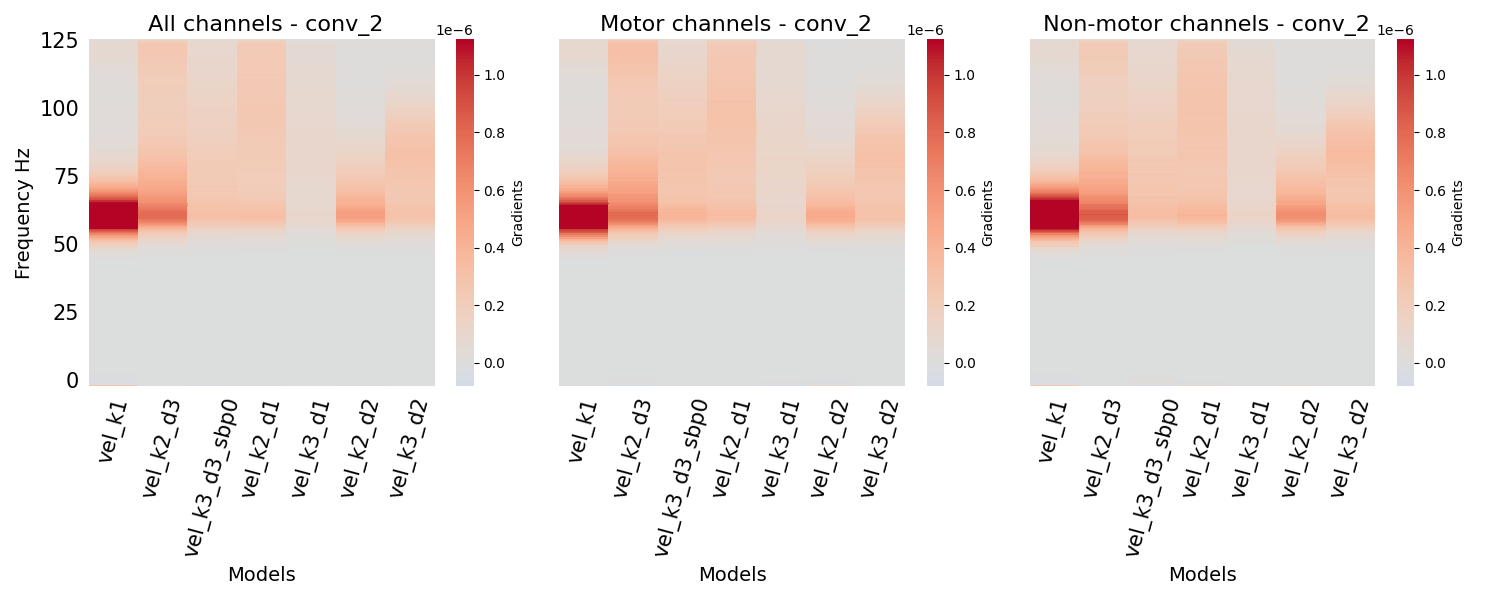
\includegraphics[width=1\linewidth]{img/appendix/A/conv-2/hp-sm/vel-model-gradients_all_kinds}
   \caption{}
   \label{fig:vel-hp-shifted-grads-conv-2}
\end{subfigure}

\begin{subfigure}[b]{\textwidth}
   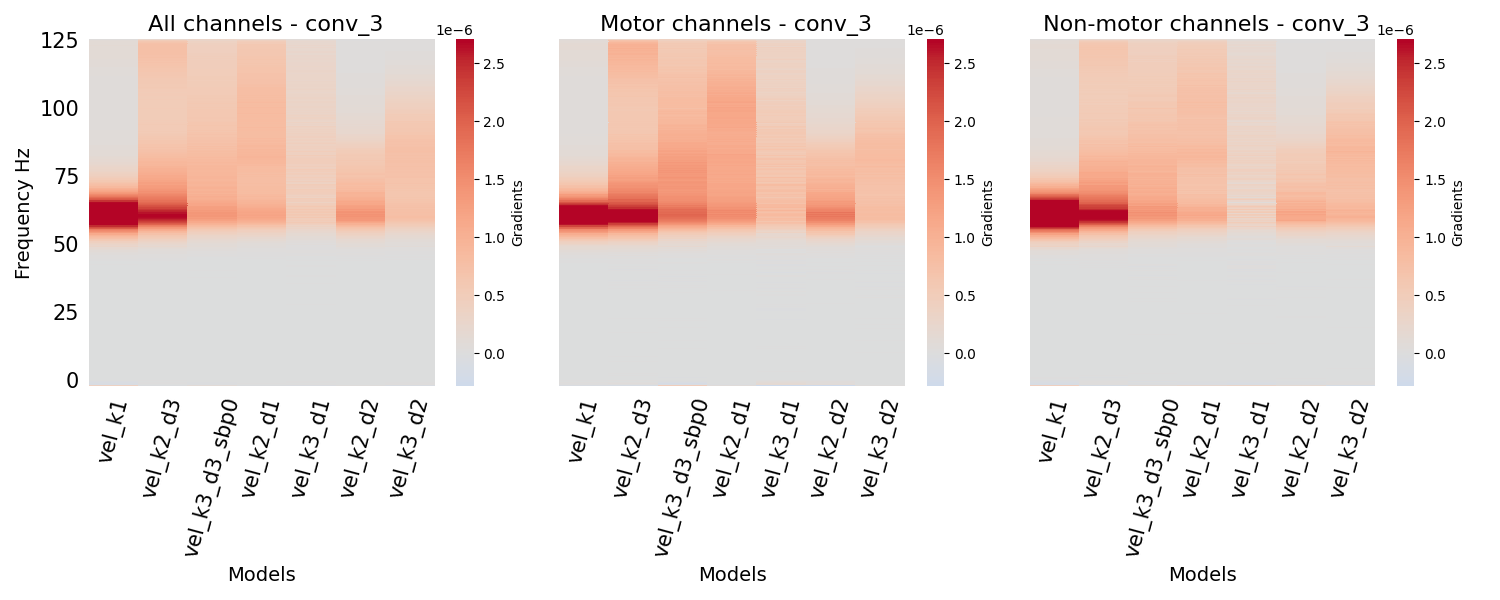
\includegraphics[width=1\linewidth]{img/appendix/A/conv-3/hp-sm/vel-model-gradients_all_kinds}
   \caption{}
   \label{fig:vel-hp-shifted-grads-conv-3}
\end{subfigure}

\end{figure}
\clearpage   

\begin{figure}[!htbp]\ContinuedFloat
\begin{subfigure}[b]{\textwidth}
   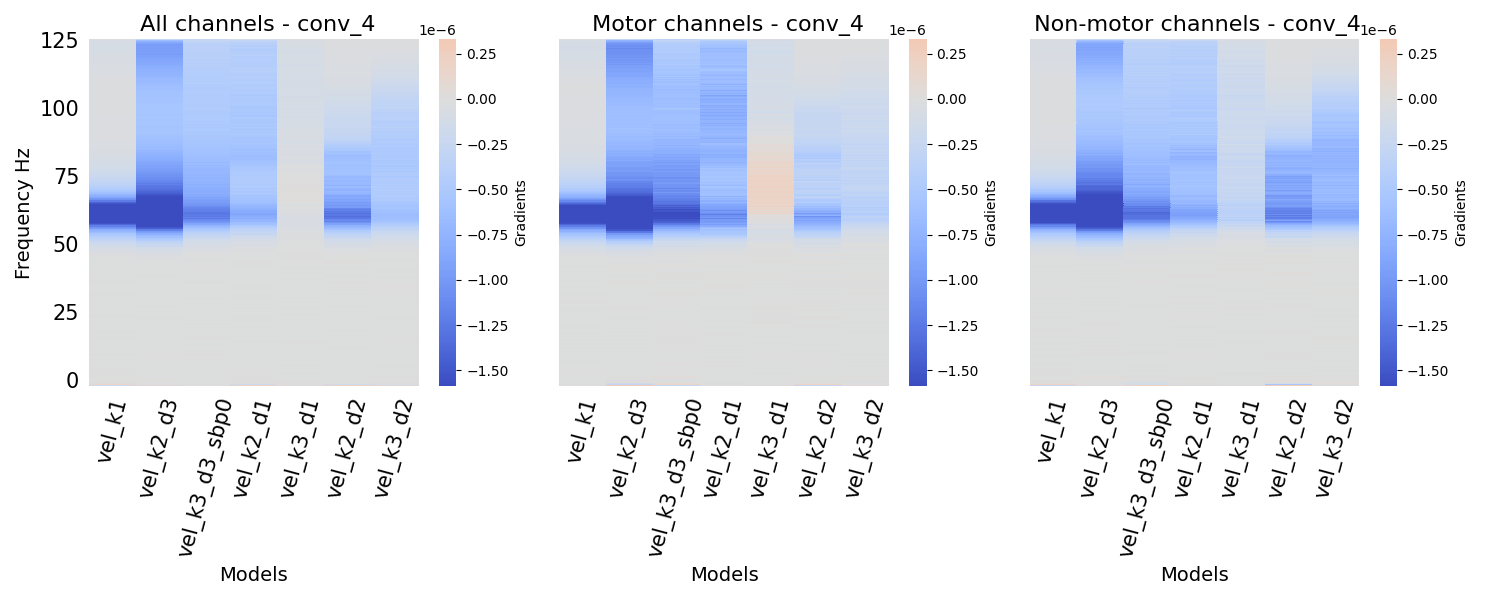
\includegraphics[width=1\linewidth]{img/appendix/A/conv-4/hp-sm/vel-model_gradients_all_kinds}
   \caption{}
   \label{fig:vel-hp-shifted-grads-conv-4}
\end{subfigure}

\begin{subfigure}[b]{\textwidth}
   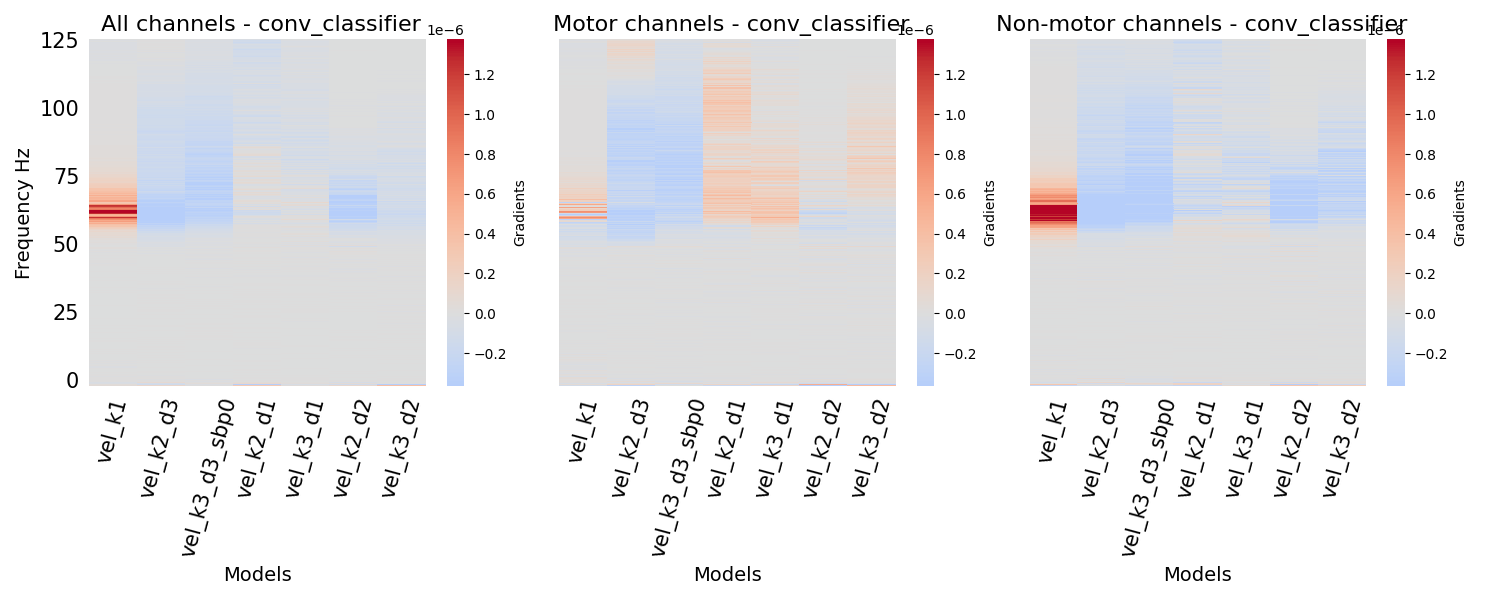
\includegraphics[width=1\linewidth]{img/appendix/A/conv-classifier/hp-sm/vel-model_gradients_all_kinds}
   \caption{}
   \label{fig:vel-hp-shifted-grads-conv-classifier}
\end{subfigure}

\caption[]{Gradients of the different CNN architectures decoding velocity from the high-passed dataset in the shifted setting (acausal prediction) (see Section~\ref{subsec:shifting-the-predicted-time-point-to-the-centre-of-the-receptive-field}. \textbf{(a)} shows gradients of the convolutional layer in the second block; \textbf{(b)} shows gradients of the convolutional layer in the third block; \textbf{(c)} shows gradients of the fourth convolutional block; \textbf{(d)} shows gradients of the last convolutional layer - the output layer. All channels include channels that do not belong to motor neither non-motor channel sets. See Section \ref{subsec:ieeg-data-preprocessing}}
\label{fig:vel-hp-shifted-grads}
\end{figure}

\clearpage
\section*{Absolute velocity}\label{sec:absolute-velocity-appendixB}

\subsection*{Full dataset}\label{subsec:absVel-full-dataset-appendixB}
\begin{figure}[!htpb]
\centering
\begin{subfigure}[b]{\textwidth}
   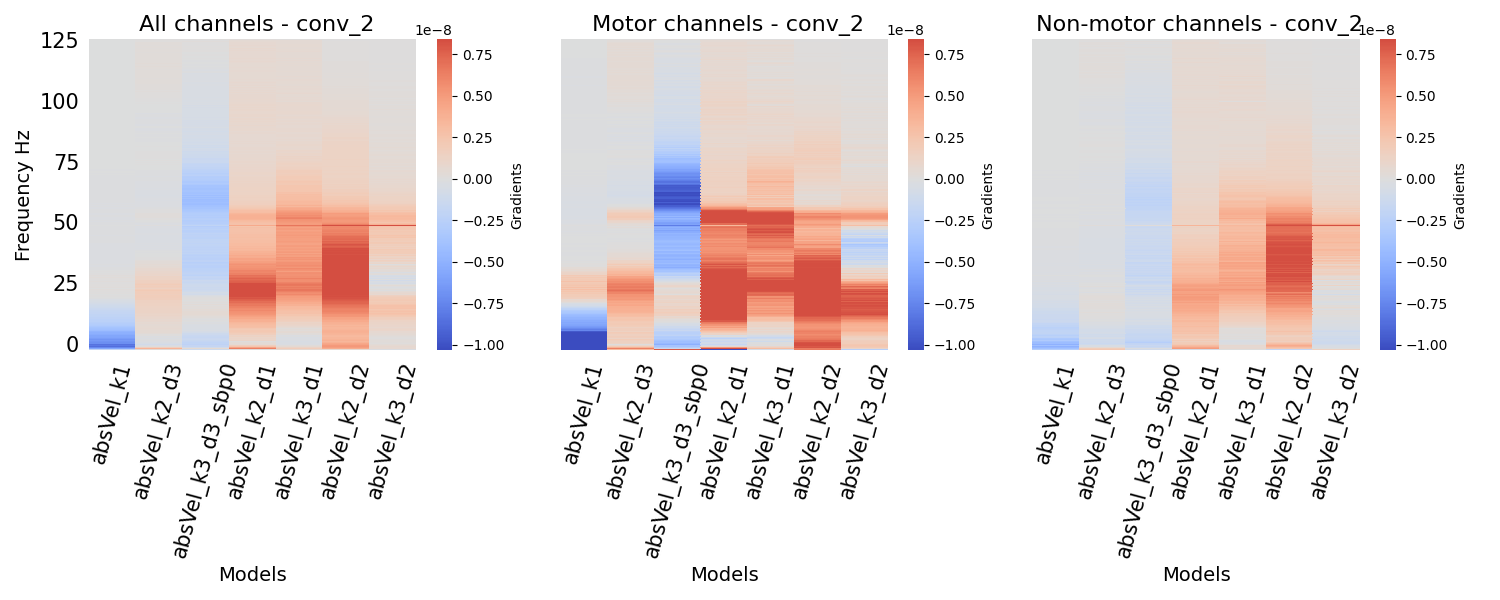
\includegraphics[width=1\linewidth]{img/appendix/A/conv-2/sm/absVel-model-gradients-all_kinds}
   \caption{}
   \label{fig:absVel-shifted-grads-conv-2}
\end{subfigure}

\begin{subfigure}[b]{\textwidth}
   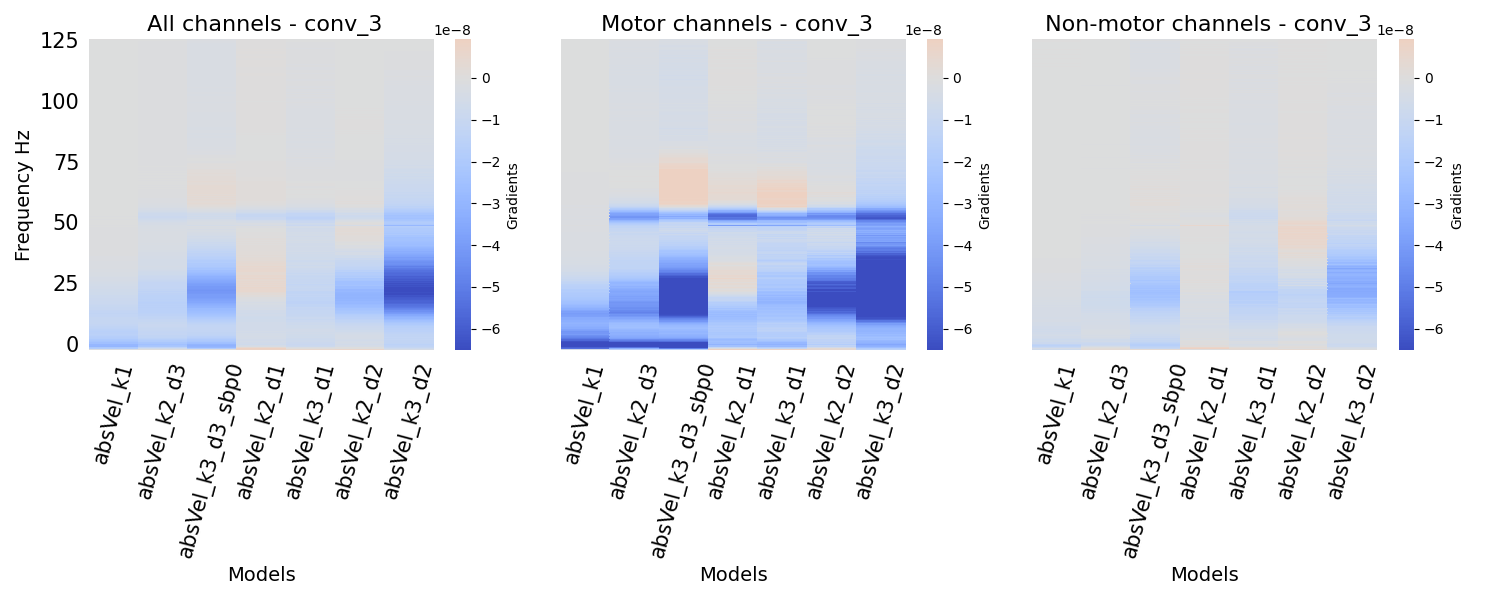
\includegraphics[width=1\linewidth]{img/appendix/A/conv-3/sm/absVel-model-gradients-all_kinds}
   \caption{}
   \label{fig:absVel-shifted-grads-conv-3}
\end{subfigure}
\end{figure}
\clearpage   

\begin{figure}[!htbp]\ContinuedFloat
\begin{subfigure}[b]{\textwidth}
   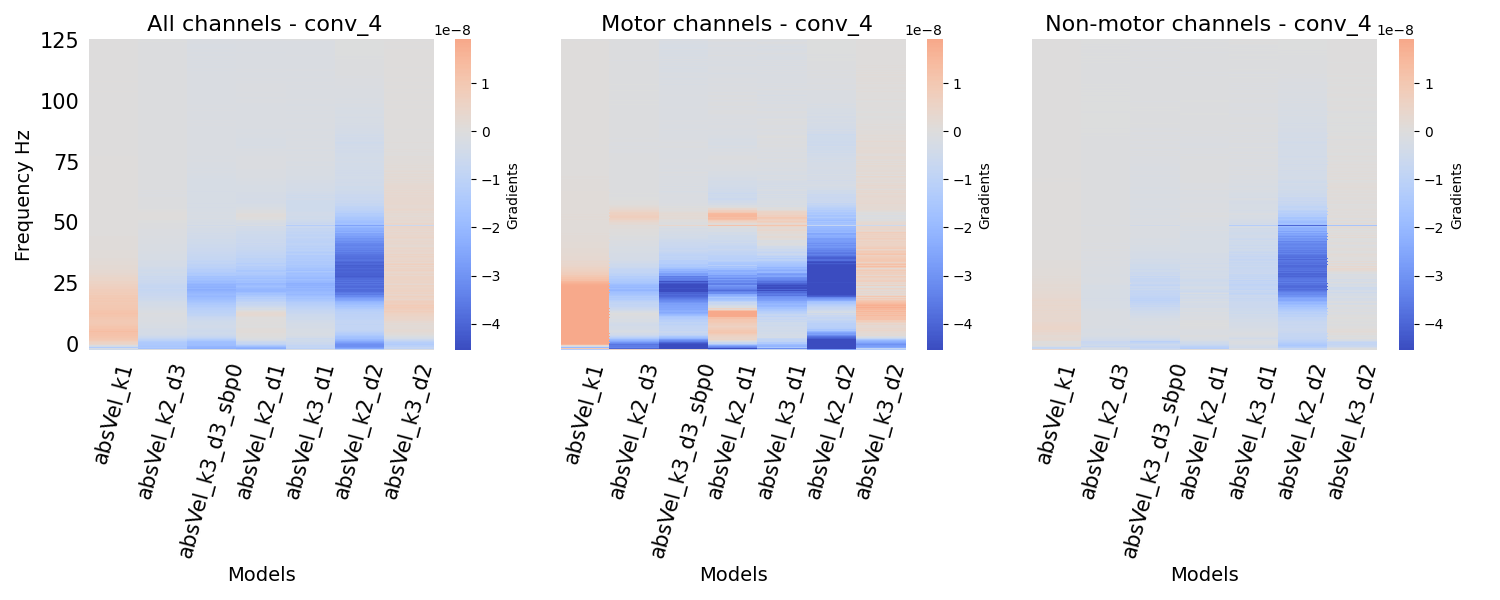
\includegraphics[width=1\linewidth]{img/appendix/A/conv-4/sm/absVel-model-gradients_all_kinds}
   \caption{}
   \label{fig:absVel-shifted-grads-conv-4}
\end{subfigure}

\begin{subfigure}[b]{\textwidth}
   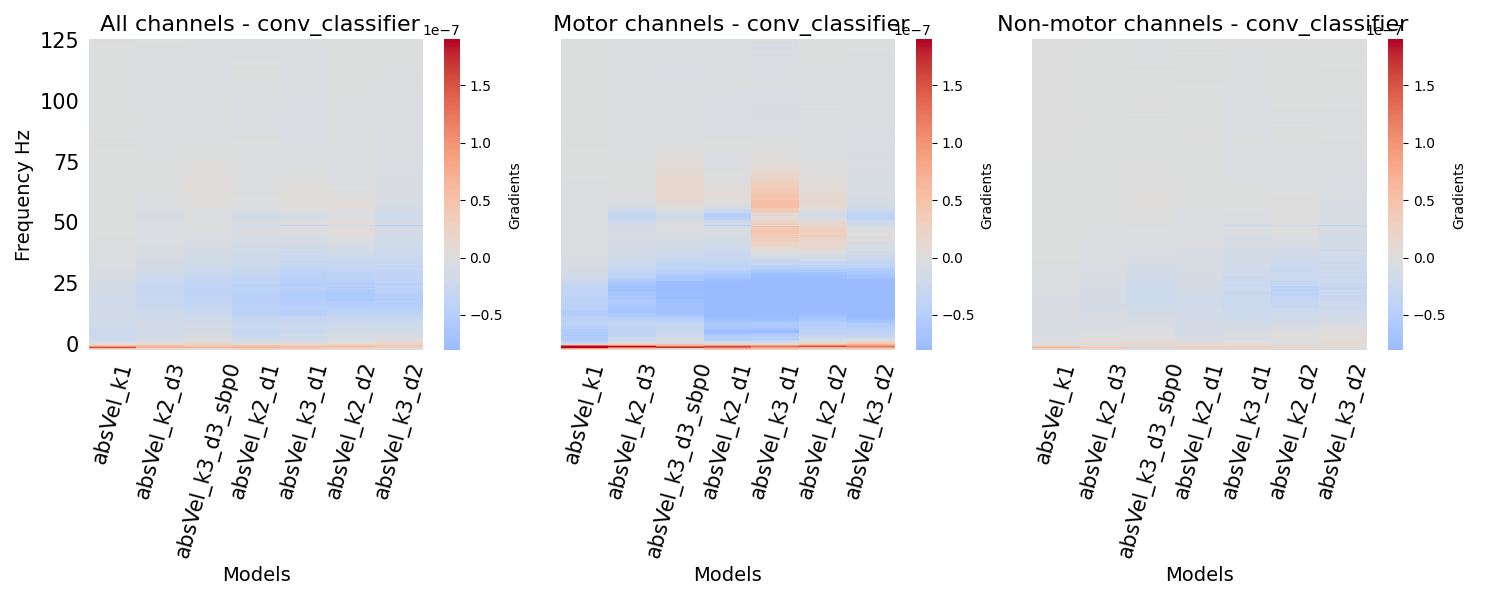
\includegraphics[width=1\linewidth]{img/appendix/A/conv-classifier/sm/absVel-model-gradients_all_kinds}
   \caption{}
   \label{fig:absVel-shifted-grads-conv-classifier}
\end{subfigure}

\caption[]{Gradients of the different CNN architectures decoding absolute velocity from the full dataset in the shifted setting (acausal prediction) (see Section~\ref{subsec:shifting-the-predicted-time-point-to-the-centre-of-the-receptive-field}. \textbf{(a)} shows gradients of the convolutional layer in the second block; \textbf{(b)} shows gradients of the convolutional layer in the third block; \textbf{(c)} shows gradients of the fourth convolutional block; \textbf{(d)} shows gradients of the last convolutional layer - the output layer. All channels include channels that do not belong to motor neither non-motor channel sets. See Section \ref{subsec:ieeg-data-preprocessing}}
\label{fig:absVel-shifted-grads}
\end{figure}

\clearpage
\subsection*{High-passed dataset}\label{subsec:absVel-high-passed-dataset-appendixB}
\begin{figure}[!htpb]
\centering
\begin{subfigure}[b]{\textwidth}
   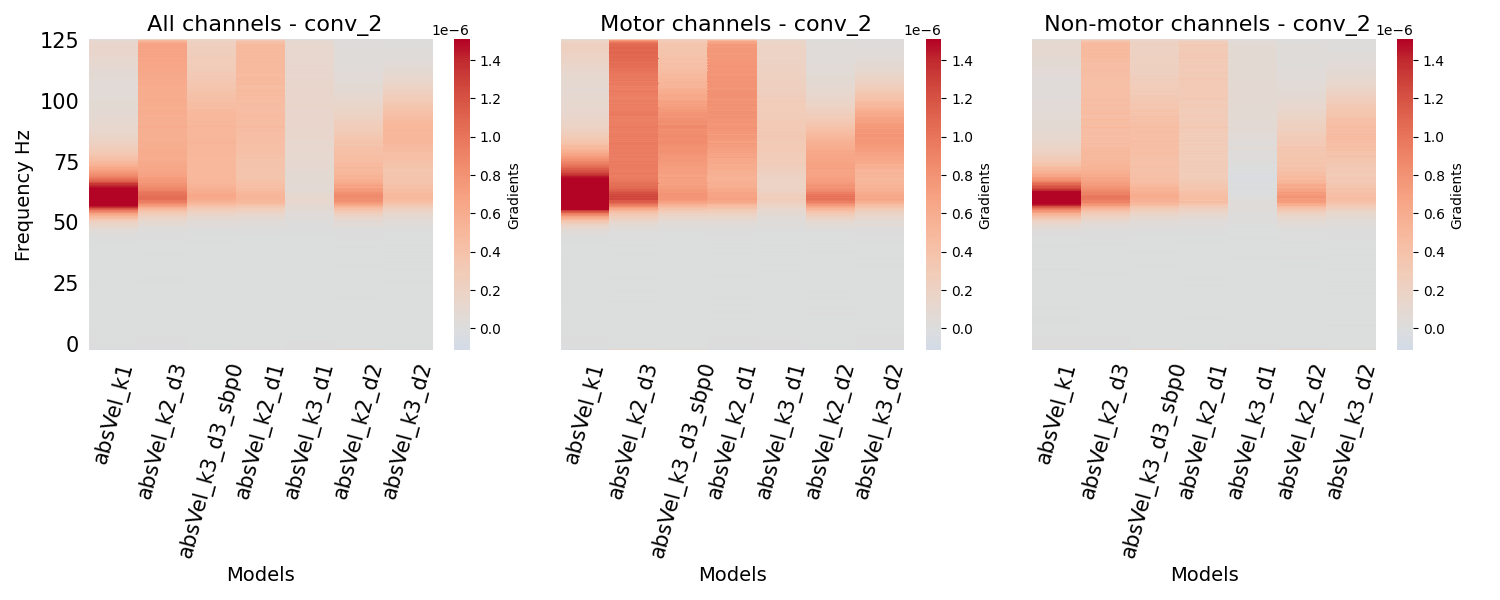
\includegraphics[width=1\linewidth]{img/appendix/A/conv-2/hp-sm/absVel-model-gradients_all_kinds}
   \caption{}
   \label{fig:absVel-hp-shifted-grads-conv-2}
\end{subfigure}

\begin{subfigure}[b]{\textwidth}
   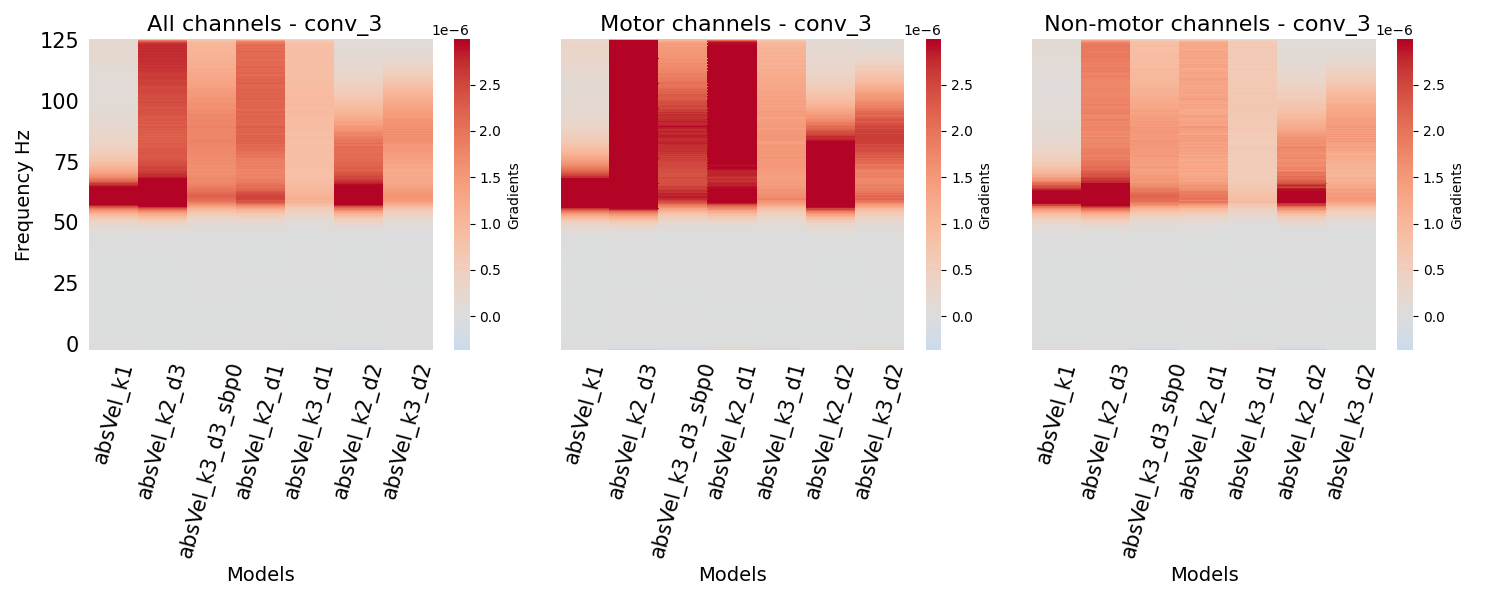
\includegraphics[width=1\linewidth]{img/appendix/A/conv-3/hp-sm/absVel-model-gradients_all_kinds}
   \caption{}
   \label{fig:absVel-hp-shifted-grads-conv-3}
\end{subfigure}
\end{figure}
\clearpage   

\begin{figure}[!htbp]\ContinuedFloat
\begin{subfigure}[b]{\textwidth}
   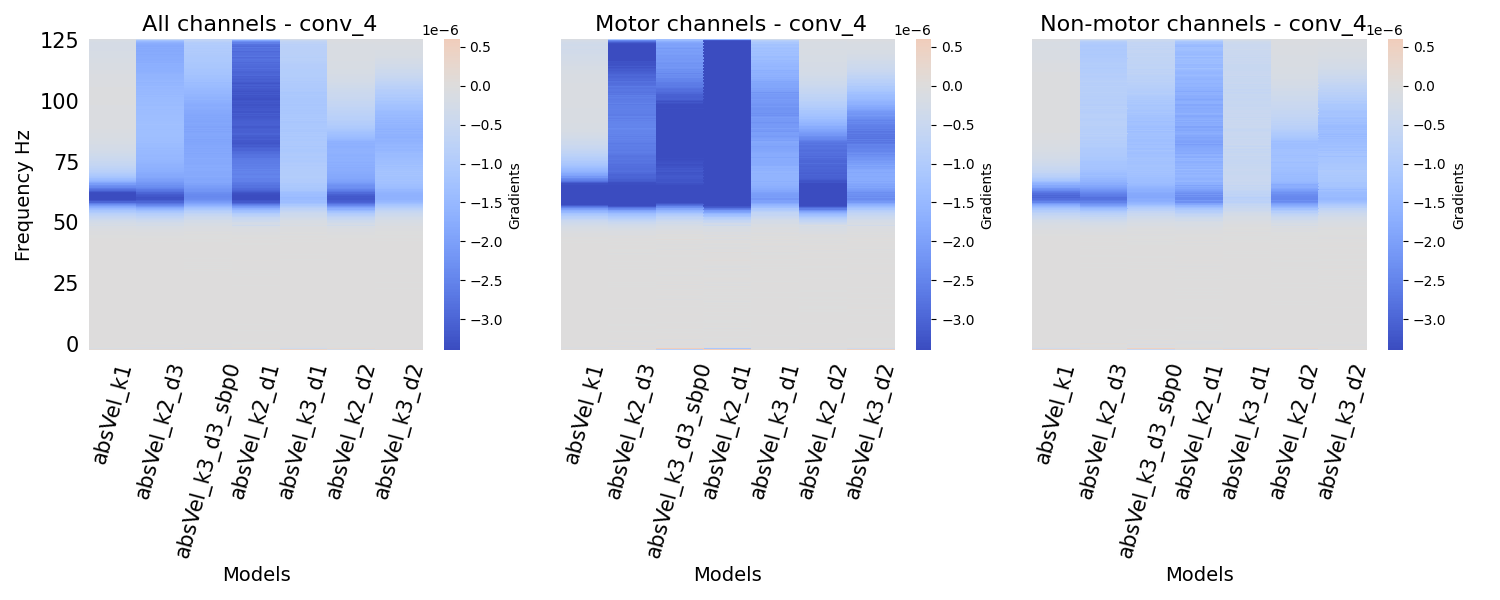
\includegraphics[width=1\linewidth]{img/appendix/A/conv-4/hp-sm/absVel-model_gradients_all_kinds}
   \caption{}
   \label{fig:absVel-hp-shifted-grads-conv-4}
\end{subfigure}

\begin{subfigure}[b]{\textwidth}
   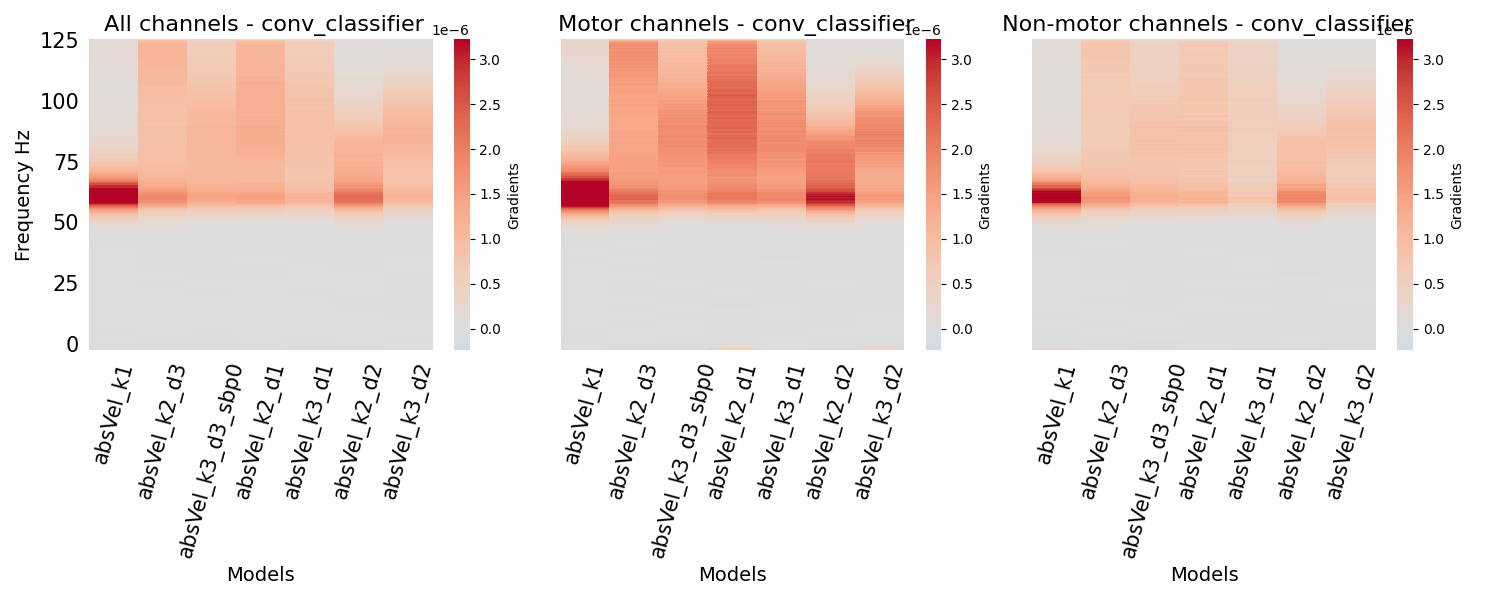
\includegraphics[width=1\linewidth]{img/appendix/A/conv-classifier/hp-sm/absVel-model_gradients_all_kinds}
   \caption{}
   \label{fig:absVel-hp-shifted-grads-conv-classifier}
\end{subfigure}

\caption[]{Gradients of the different CNN architectures decoding absolute velocity from the high-passed dataset in the shifted setting (acausal prediction) (see Section~\ref{subsec:shifting-the-predicted-time-point-to-the-centre-of-the-receptive-field}. \textbf{(a)} shows gradients of the convolutional layer in the second block; \textbf{(b)} shows gradients of the convolutional layer in the third block; \textbf{(c)} shows gradients of the fourth convolutional block; \textbf{(d)} shows gradients of the last convolutional layer - the output layer. All channels include channels that do not belong to motor neither non-motor channel sets. See Section \ref{subsec:ieeg-data-preprocessing}}
\label{fig:absVel-hp-shifted-grads}
\end{figure}